\documentclass[11pt]{article}
\usepackage[paperwidth=12cm, paperheight=18cm, margin=1cm]{geometry}
\usepackage{amsmath, tikz}
\pagestyle{empty}

\begin{document}
\begin{center}
  {\LARGE\bfseries The Central Limit Theorem}\\[4pt]
  {\large Add up dice and a bell curve appears}
\end{center}

One die is flat: every face has probability \(\tfrac16\).
Add three dice together and the sum is already bell-shaped.

\section*{The theorem}
For independent \(X_i\) with mean \(\mu\) and variance \(\sigma^2\):
\[
  \frac{\bar X_n - \mu}{\sigma / \sqrt{n}}
  \xrightarrow{\;d\;} \mathcal{N}(0, 1)
\]

\section*{Sum of three dice}
\[
  \mu = 3 \cdot 3.5 = 10.5, \qquad \sigma^2 = 3 \cdot \frac{35}{12} = 8.75
\]

\begin{center}
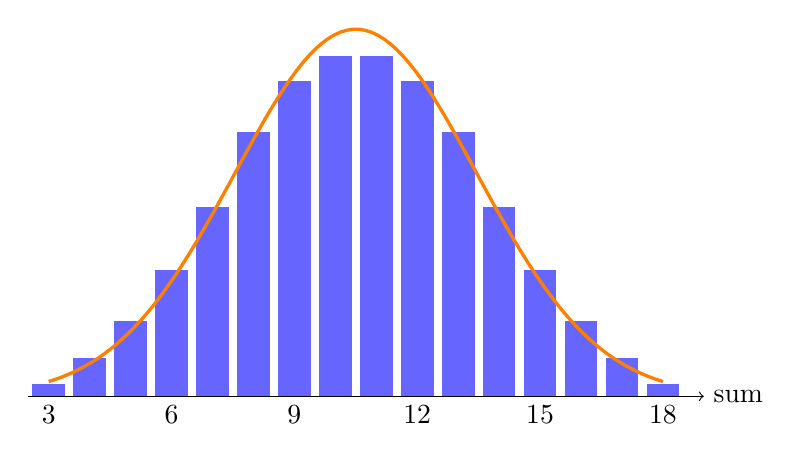
\begin{tikzpicture}[xscale=0.52, yscale=0.16]
  \draw[->] (2.5,0) -- (19,0) node[right] {sum};
  \foreach \s/\c in {3/1, 4/3, 5/6, 6/10, 7/15, 8/21, 9/25, 10/27,
                     11/27, 12/25, 13/21, 14/15, 15/10, 16/6, 17/3, 18/1}
    \fill[blue!60] (\s-0.4,0) rectangle (\s+0.4,\c);
  \foreach \s in {3, 6, ..., 18} \node[below] at (\s,0) {\s};
  \draw[orange, very thick, domain=3:18, samples=100]
    plot (\x, {216 * exp(-(\x-10.5)^2/17.5) / sqrt(2*pi*8.75)});
\end{tikzpicture}
\end{center}

Bars: the exact counts out of \(6^3 = 216\) rolls.
Curve: the normal approximation.

\centerline{\bfseries Averages of almost anything become normal.}
\end{document}
